\documentclass[]{book}

%These tell TeX which packages to use.
\usepackage{array,epsfig}
\usepackage{amsmath}
\usepackage{amsfonts}
\usepackage{amssymb}
\usepackage{amsxtra}
\usepackage{amsthm}
\usepackage{mathrsfs}
\usepackage{color}
\usepackage{mathtools}
\usepackage{hyperref}
\usepackage{cleveref}

%Here I define some theorem styles and shortcut commands for symbols I use often
\theoremstyle{definition}
\newtheorem{defn}{Definition}
\newtheorem{thm}{Theorem}
\newtheorem{cor}{Corollary}
\newtheorem*{rmk}{Remark}
\newtheorem{lem}{Lemma}
\newtheorem*{joke}{Joke}
\newtheorem{ex}{Example}
\newtheorem*{soln}{Solution}
\newtheorem{prop}{Proposition}

\newcommand{\lra}{\longrightarrow}
\newcommand{\ra}{\rightarrow}
\newcommand{\surj}{\twoheadrightarrow}
\newcommand{\graph}{\mathrm{graph}} \newcommand{\bb}[1]{\mathbb{#1}}
\newcommand{\Z}{\bb{Z}} \newcommand{\Q}{\bb{Q}} \newcommand{\R}{\bb{R}}
\newcommand{\C}{\bb{C}} \newcommand{\N}{\bb{N}} \newcommand{\M}{\mathbf{M}}
\newcommand{\m}{\mathbf{m}} \newcommand{\MM}{\mathscr{M}}
\newcommand{\HH}{\mathscr{H}}
\newcommand{\Om}{\Omega}
\newcommand{\Ho}{\in\HH(\Om)}
\newcommand{\bd}{\partial}
\newcommand{\del}{\partial}
\newcommand{\bardel}{\overline\partial}
\newcommand{\textdf}[1]{\textbf{\textsf{#1}}\index{#1}}
\newcommand{\img}{\mathrm{img}}
\newcommand{\ip}[2]{\left\langle{#1},{#2}\right\rangle}
\newcommand{\inter}[1]{\mathrm{int}{#1}}
\newcommand{\exter}[1]{\mathrm{ext}{#1}} \newcommand{\cl}[1]{\mathrm{cl}{#1}}
\newcommand{\ds}{\displaystyle}
\newcommand{\vol}{\mathrm{vol}} \newcommand{\cnt}{\mathrm{ct}}
\newcommand{\osc}{\mathrm{osc}} \newcommand{\LL}{\mathbf{L}}
\newcommand{\UU}{\mathbf{U}} \newcommand{\support}{\mathrm{support}}
\newcommand{\AND}{\;\wedge\;}
\newcommand{\OR}{\;\vee\;}
\newcommand{\Oset}{\varnothing}
\newcommand{\st}{\ni}
\newcommand{\wh}{\widehat}
\newcommand{\XX}{\mathbf{X}} \newcommand{\YY}{\mathbf{Y}}
\newcommand{\TT}{\mathcal{T}} \newcommand{\WW}{\mathbf{W}}

\DeclareMathOperator*{\argmax}{arg\,max}
\DeclareMathOperator*{\argmin}{arg\,min} \DeclareMathOperator*{\Cov}{Cov}
\DeclareMathOperator*{\EPE}{EPE} \DeclareMathOperator*{\Var}{Var}
\DeclareMathOperator*{\Bias}{Bias} \DeclareMathOperator*{\tr}{trace}
\DeclareMathOperator*{\RSS}{RSS} \DeclareMathOperator*{\WRSS}{WRSS}
\DeclareMathOperator*{\diag}{diag}


%Pagination stuff.
\setlength{\topmargin}{-.3 in}
\setlength{\oddsidemargin}{0in}
\setlength{\evensidemargin}{0in}
\setlength{\textheight}{9.in}
\setlength{\textwidth}{6.5in}
\pagestyle{empty}



\begin{document}


\begin{center}
	{\Large Elements of Statistical Learning, Solutions}\\
	Marios\\ %You should put your name here
\end{center}

\vspace{0.2 cm}


\subsection*{Exercises for Section 2}

\begin{enumerate}
	\item\label{ex:k-classes} Suppose each of $K$-classes has an associated
	target $t_k$, which is a vector of all zeros, except a one in the $k$th
	position. Show that classifying to the largest element of $\hat{y}$ amounts
	to choosing the closest target, $\min_k\|t_k-\hat{y}\|$, if the elements of
	$\hat{y}$ sum to one.
	\begin{soln}
		\newcommand{\normone}[1]{\sum_{i\ne #1}|\hat{y}_i|+|1-\hat{y}_{#1}|} Let
		$k^*=\argmax_k \hat{y}_k$ and suppose that there is $k'\le k^*$ such
		that $\|t_{k'}-\hat{y}\| < \|t_{k^*}-\hat{y}\|$.
		\begin{itemize}
			\item $\ell_1$ norm. It holds that
			      $\|t_k-\hat{y}\|_1=\sum_i|t_{k,i}-\hat{y}_i|=\sum_{i\ne
					      k}|\hat{y}_i|+|1-\hat{y}_k|$. Hence, we get
			      \begin{equation}\label{2.1-inequality}
				      \normone{k'} < \normone{k^*}\Rightarrow |\hat{y}_{k^*}|-|1-\hat{y}_{k^*}|
				      < |\hat{y}_{k'}|-|1-\hat{y}_{k'}|.
			      \end{equation}
			      But the function $f(y)=|y|-|1-y|$ is increasing in $[0,1]$
			      hence~\Cref{2.1-inequality} implies that
			      $\hat{y}_{k^*}<\hat{y}_{k'}$, reaching a contradiction.
			\item $\ell_2$ norm. Similarly, we get that
			      $\hat{y}_{k^*}(1-\hat{y}_{k^*})<\hat{y}_{k'}(1-\hat{y}_{k'})$
			      and since the function $f(y)=y(1-y)$ is increasing in $[0,1]$,
			      we get that $\hat{y}_{k^*}<\hat{y}_{k'}$, reaching a
			      contradiction.
		\end{itemize}
	\end{soln}

	\item\label{ex:exact-distribution} Show how to compute the Bayes decision
	boundary for the simulation example in Figure 2.5.
	\begin{soln}
		If we know the exact probability distribution $\Pr[G,X]$,
		$X\in\mathbb{R}^p$, $G\in \mathcal{G}=\{B,O\}$, then we can probably
		also derive $f(X)=\Pr[B|X]=\Pr[B,X]/\Pr[X]$, namely the probability that
		$X$ maps to blue in reality. This assume that we also know $\Pr[X]$
		which is not necessary. Of course, $\Pr[O|X]=1-\Pr[B|X]$. So now, all we
		have to do is to check for each $x\in\mathbb{R}^p$, whether $f(x)>1/2$.
		For the case where $x\in\mathbb{R}$, this is trivial. We simply solve
		the equation $f(x)=1/2$. This also hold in general. So the points (in
		$\mathbb{R}$), the line (in $\mathbb{R}^2$), and the $(p-1)$-dimensional
		hyperplane (in $\mathbb{R}^p$), is the solution to the equation
		$f(x)=\Pr[B|X]=1/2$. See Figure~\ref{fig:exercise2.2} for another
		example.

		\begin{figure}[ht]
			\label{fig:exercise2.2}
			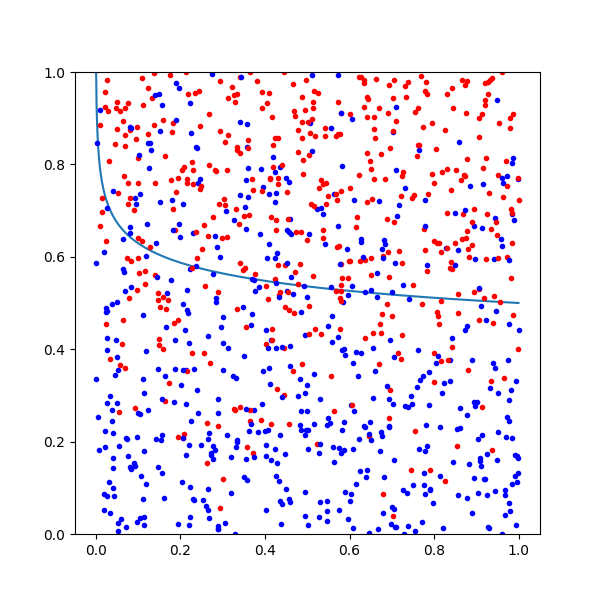
\includegraphics[width=8cm]{plots/ex22.png}
			\centering
			\caption{In this example we have computed the Bayes decision
			boundary when $X\sim U(0,1)^2$ and
			$\Pr[Y=\text{red}|X]=X_1^{1/10}X_2$. Therefore, the line is the
			solution to the equation $X_1^{1/10}X_2=1/2$.}
		\end{figure}
	\end{soln}

	\item\label{ex:eq2.24} Derive equation 2.24. Consider $N$ data points
	uniformly sampled in a $p$-dimensional unit ball centered at the origin.
	Show that the median distance from the origin to the closest data point is
	given by the expression $$d(p,N)=\left(1-\frac{1}{2}^{1/N}\right)^{1/p}.$$
	\begin{soln}
		We start with the cumulative distribution function (CDF) of the distance
		of a random point from the origin. The volume of a $p$-dimensional ball
		of radius $d$ is $V_p(d)=c_pd^p$, where $c_p$ is a value that does not
		depend on $d$. Therefore,
		\begin{equation}\tag{First trick to remember}
			F_D(d)=\Pr[D\le d]=\frac{V_p(d)}{V_p(1)}=d^p.
		\end{equation}
		Now it is useful to compute the CDF of the distance of the closest point
		$C=\min_{i\in[N]} D_i$. We have that
		\begin{equation}
			\begin{split}
				F_C(d) &= \Pr[C\le d] \\
				&= 1-\Pr[C\ge d] \\
				&= 1-\Pr\left[\min_{i\in[N]} D_i \ge d\right] \\
				&= 1-\Pr[\forall i\in[N], D_i \ge d] \\
				&= 1-\prod_{i\in[N]}\Pr[D_i \ge d] \\
				&= 1-\Pr[D \ge d]^N \\
				&= 1-(1-\Pr[D \le d])^N \\
				&= 1-(1-d^p)^N.
			\end{split}
		\end{equation}
		By definition, the median $m$ is defined as $F_C(m)=1/2$. Hence, we get
		that $(1-m^p)^N=1/2$ and solving for $m$, we get
		\[m=\left(1-\frac{1}{2}^{1/N}\right)^{1/p}.\]
	\end{soln}

	\item\label{ex:multi-normal} Consider inputs drawn from a spherical
	multinormal distribution $X\sim N(0,\mathbf{I}_p)$. The squared distance
	from any sample point to the origin has a $\chi_p^2$ distribution with mean
	$p$. Consider a prediction point $x_0$ drawn from this distribution, and let
	$a=x_0/\|x_0\|$ be an associated unit vector. Let $z_i=a^Tx_i$ be the
	projection of each of the training points on this direction.

	Show that the $z_i$ are distributed according to $N(0,1)$ with expected
	squared distance from the origin $1$, while the target point has expected
	squared distance $p$ from the origin.

	\begin{soln}
		We use the fact that for any $a\in\mathbb{R}^p$, if $x\sim
			N(0,\mathbf{I}_p)$, then $a^Tx\sim
			N\left(\sum_ja_j\mu_j,\sum_ja_j^2\sigma_j^2\right)$, where
		$\mu_j=E(x_j)$ and $\sigma_j=V(x_j)$ and $j\in[p]$. Since
		$\sigma_j=1$ and $\mu_j=0$, we get that $a^Tx\sim
			N\left(0,\sum_ja_j^2\right)$. Given that $\|a\|$ is a unit vector,
		we get that $a^Tx\sim N\left(0,1\right)$. Hence
		$|z|=|a^Tx|\sim\chi_1^2$ and $E[|z|]=1$.
	\end{soln}

	\item\label{ex:eq2.27} Suppose that we know that the true relationship
	between $Y$ and $X$ is linear,
	\begin{equation}
		Y=X^T\beta+\varepsilon, \tag{2.26}
	\end{equation}
	where $\varepsilon\sim N(0,\sigma^2)$ and we fit the model by least squares
	to the training data. For an arbitrary test point $x_0$, we have $\hat
		y_0=x_0^T\hat\beta$, which can be written as $\hat y_0=x_0^T\beta +
		\sum_{i-1}^N\ell_i(x_0)\varepsilon_i$, where $\ell_i(x_0)$ is the $i$th
	element of $\XX(\XX^T\XX)^{-1}x_0$. Show that
	\[
		\EPE(x_0)=\sigma^2+E_\TT x_0^T(\XX^T\XX)^{-1}x_0\sigma^2+0^2 \tag{2.27},\]
	where you can use the fact that for any $\XX$,
	\[\Cov[\hat \beta]=(\XX^T\XX)^{-1}\sigma^2. \label{eq:cov}\tag{3.8}\]
	Additionally, suppose $N$ is large and $\TT$ were selected at random.
	Assuming $E(X)=0$, then $\XX^T\XX\to N\Cov(X)$. Show that
	\begin{equation*}
		\begin{split}
			E_{x_0}\EPE(x_0) &\approx E_{x_0}x_0^T \Cov[X]^{-1}x_0\sigma^2/N + \sigma^2\\
			&=\tr[\Cov[X]^{-1}\Cov[x_0]]\sigma^2/N+\sigma^2 \\
			&=\sigma^2(p/N)+\sigma^2.
		\end{split}\tag{2.28}
	\end{equation*}
	Make use of the cyclic property of the trace operator ($\tr(AB)=\tr(BA)$),
	and its linearity (which allows us to interchange the order of trace and
	expectation).

	\begin{soln}
		{ \newcommand{\Exp}{E_{\TT,\varepsilon}} In the first question, the test
			point $x_0$ is arbitrary and not sampled from the distribution. Thus
			the randomness is only over:
			\begin{itemize}
				\item the samples $\TT$,
				\item the error $\varepsilon$.
			\end{itemize}
			In the second part, we also sample $x_0$ and hence we consider the
			expectation of $\EPE(x_0)$.
			\begin{enumerate}
				\item We start by showing that the expected prediction error
				      equals the sum of the variance of the system, the variance
				      of the model and the squared bias of the model:
				      \begin{equation*}
					      \begin{split}
						      \EPE(x_0) &= \Exp[(y_0-\hat y_0)^2] \\
						      &= \Exp[y_0^2-2y_0\hat y_0 + \hat y_0^2] \\
						      &= \Exp[y_0^2]-2\Exp[y_0\hat y_0] + \Exp[\hat y_0^2] \\
						      &= \Exp[y_0^2]-2x_0^T\beta\Exp[\hat y_0] + \Exp[\hat y_0^2] \\
						      &= \Exp[y_0^2]\boxed{-\Exp[y_0]^2+\Exp[y_0]^2}-2x_0^T\beta\Exp[\hat y_0] + \Exp[\hat y_0^2] - \boxed{\Exp[\hat y_0]^2 + \Exp[\hat y_0]^2} \\
						      &= \Var[y_0] + \Var[\hat y_0] + \left(\Exp[\hat y_0]-x_0^T\beta\right)^2,
					      \end{split}
				      \end{equation*}
				      where the third line follows from the fact that
				      \[\Exp[y_0\hat y_0]=\Exp[(x_0^T\beta+\varepsilon)\hat
						      y_0]=x_0^T\beta\Exp[\hat y_0]+\Exp[\varepsilon\hat
						      y_0]\] and $\Exp[\varepsilon\hat
						      y_0]=\Exp[\varepsilon]\Exp[\hat y_0]=0$, since
				      $\varepsilon$ is independent from $\hat y_0$. Now,
				      we have that $\Var[y_0]=\sigma^2$. Moreover,
				      \begin{equation}
					      \begin{split}
						      \Exp[\hat y_0] &= \Exp\left[x_0^T\beta + \sum_{i-1}^N\ell_i(x_0)\varepsilon_i\right] \\
						      &= x_0^T\beta + \sum_{i-1}^N\Exp[\ell_i(x_0)\varepsilon_i] \\
						      &= x_0^T\beta + \sum_{i-1}^N\Exp[\ell_i(x_0)]\Exp[\varepsilon_i] \\
						      &= x_0^T\beta,
					      \end{split}
				      \end{equation}
				      since $\varepsilon_i$ is independent of $x_0$ and $\XX$.
				      Hence, $\Bias(\hat y_0)=\left(\Exp[\hat
						      y_0]-x_0^T\beta\right)=0$. Last, we want to calculate the
				      variance of our prediction $\Var[\hat y_0]$. We have
				      \begin{equation}
					      \begin{split}
						      \Var[\hat y_0] &= \Var[x_0^T\hat\beta] \\
						      &= x_0^T\Cov[\hat\beta]x_0 \\
						      &= x_0^T(\XX^T\XX)^{-1}\sigma^2x_0,
					      \end{split}
				      \end{equation}
				      where the last line comes from~\cref{eq:cov}.
				\item Now we have that
				      \begin{equation}
					      \begin{split}
						      E_{x_0}\EPE(x_0) &\approx E_{x_0}[x_0^T \Cov[X]^{-1}x_0]\sigma^2/N + \sigma^2 \\
						      &= E_{x_0}[\tr[x_0^T \Cov[X]^{-1}x_0]]\sigma^2/N + \sigma^2 \\
						      &= E_{x_0}[\tr[\Cov[X]^{-1}x_0x_0^T]]\sigma^2/N + \sigma^2 \\
						      &= \tr[E_{x_0}[\Cov[X]^{-1}x_0x_0^T]]\sigma^2/N + \sigma^2 \\
						      &= \tr[\Cov[X]^{-1}E_{x_0}[x_0x_0^T]]\sigma^2/N + \sigma^2 \\
						      &= \tr[\Cov[X]^{-1}\Cov[x_0]]\sigma^2/N + \sigma^2 \\
						      &= \tr[\mathbf{I}_p]\sigma^2/N + \sigma^2 \\
						      &= p\sigma^2/N + \sigma^2
					      \end{split}
				      \end{equation}
			\end{enumerate}
		} We see that the function
		$f(p)=E_{x_0}\EPE(x_0)=\sigma^2(p/N)+\sigma^2$ increases linearly with
		$p$, with slope $f'(p)=\sigma^2/N$. Hence as long as we have
		sufficiently many samples $N$ this increase becomes negligible. In other
		words, even if we have a lot of dimensions, the expected $\EPE$ remains
		constant. Of course, the reason is that we imposed heavy restrictions on
		the class of models being fitted.
	\end{soln}

	\item\label{ex:2.6} Consider a regression problem with inputs $x_i$ and
	outputs $y_i$, and a parameterized model $f_\theta(x)$ to be fit by least
	squares. Show that if there are observations with \emph{tied} or
	\emph{identical} values of $x$, then the fit can be obtained from a reduced
	weighted least squares problem.

	\begin{soln}
		The weighted least squares problem is defined as the problem of
		minimizing the value
		\[\WRSS\nolimits_{(x_i,y_i,w_i)}(\beta)=\sum_{i=1}^Nw_i(y_i-\hat
			f_\beta(x_i))^2.\] It generasizes $\RSS$ since by setting $w_i=1$ we get
		the $\RSS$. The idea behind $\WRSS$ is that some pairs $(x_i,y_i)$ may
		have errors and some may be more accurate. By giving them weights, we
		reward the more accurate ones and we penalize the less accurate.

		A reduced least squares problem is one that uses fewer observations than
		available; $N'<N$.

		Suppose that we have $N$ observations $(x_i,y_i)$ with some of them
		sharing the same $x_i$. Suppose we have $N'$ distinct $x_i$s and for
		each distinct $x_i$, we have $N_i$ observations, so
		$N=\sum_{i=1}^{N'}N_i$. We wish to compute the value $\argmin_\beta
			\RSS(\beta)$. We will show that
		\[\argmin_\beta \RSS\nolimits_{(x_i,y_i)}(\beta)=\argmin_\beta
			\WRSS\nolimits_{(x_i,\overline y_i,N_i)}(\beta).\] We have{
				\newcommand{\fx}{\hat f_\beta(x_i)}
				\newcommand{\fs}{\hat f^2_\beta(x_i)}
				\begin{equation}
					\begin{split}
						\argmin_\beta \RSS\nolimits_{(x_i,y_i)}(\beta) &=
						\argmin_\beta\sum_{i=1}^N(y_i-\fx)^2 \\
						&= \argmin_\beta\sum_{i=1}^{N'}\sum_{j=1}^{N_i}(y_i-\fx)^2 \\
						&= \argmin_\beta\sum_{i=1}^{N'}\sum_{j=1}^{N_i}(y_i^2-2y_i\fx + \fs) \\
						&= \argmin_\beta\sum_{i=1}^{N'}\sum_{j=1}^{N_i}(-2y_i\fx + \fs) \\
						&= \argmin_\beta\sum_{i=1}^{N'}(-2N_i\overline y_i\fx + N_i\fs)\\
						&= \argmin_\beta\sum_{i=1}^{N'}N_i(-2\overline y_i\fx + \fs)\\
						&= \argmin_\beta\sum_{i=1}^{N'}N_i(\overline y_i^2-2\overline y_i\fx + \fs)\\
						&= \argmin_\beta\sum_{i=1}^{N'}N_i(\overline y_i-\fx)^2 \\
						&= \argmin_\beta\WRSS\nolimits_{(x_i,\overline y_i,N_i)}(\beta),
					\end{split}
				\end{equation}}
		where the fourth and the seventh lines come from the fact that for any
		function $f$ and $c\in\mathbb R$, it holds that $\argmin_\beta (f(\beta)+c)=\argmin_\beta{f(\beta)}$.
	\end{soln}

	\item Suppose we have a sample of $N$ pairs $x_i,y_i$ drawn i.i.d from the
	      distribution characterized as follows:
	      \begin{itemize}
		      \item[] $x_i\sim h(x)$, the design density
		      \item[] $y_i=f(x_i)+\varepsilon_i$, $f$ is the regression function
		      \item[] $\varepsilon_i\sim(0,\sigma^2)$ (mean zero, variance $\sigma^2$)
	      \end{itemize}
	      We construct an estimator for $f$ \emph{linear} in the $y_i$,
	      \[\hat f(x_0)=\sum_{i=1}^N\ell_i(x_0;\mathcal{X})y_i,\] where the weights
	      $\ell_i(x_0;\mathcal{X})$ do not depend on the $y_i$, but do depend on the
	      entire training sequence of $x_i$, denoted here by $\mathcal{X}$.
	      \begin{enumerate}
		      \item Show that the linear regression and $k$-nearest-neighbor
		            regression are members of this class of estimators. Describe explicitly
		            the weights $\ell_i(x_0;\mathcal{X})$ in each of these cases.
		      \item Decompose the conditional mean-squared error
		            \[E_{\mathcal{Y}|\mathcal{X}}(f(x_0)-\hat f(x_0))^2\] into a conditional
		            squared bias and a conditional variance component. Like $\mathcal{X}$,
		            $\mathcal{Y}$ represents the entire training sequence of $y_i$.
		      \item Decompose the mean-squared error $E_{\mathcal{X,Y}}(f(x_0)-\hat
			            f(x_0))^2$ into a squared bias and a variance component.
		      \item Establish a relationship between the squared biases and variances
		            in the above two cases.
	      \end{enumerate}

	      \begin{soln}{
			      \renewcommand{\XX}{\mathcal{X}}
			      \renewcommand{\YY}{\mathcal{Y}}
			      \begin{enumerate}
				      \item For linear regression, we have that $\hat f(x_0) =
					            x^T(\XX^T\XX)^{-1}\XX y=\sum_{i=1}^N\ell_i(x_0;\XX)y_i$, where
				            $\ell_i(x_0;\XX)$ is the $i$th element of the vector
				            $x^T(\XX^T\XX)^{-1}\XX$. For the $k$-nearest neighbor, we have that
				            $\ell_i(x_0;\XX)=\frac{1}{k}I(x_i\in N_k(x_0,\XX))$, where
				            $N_k(x_0,\XX)$ is the set of the $k$ closest points to $x_0$.

				      \item We have that
				            \begin{equation}
					            \begin{split}
						            E_{\YY/\XX}[(f(x_0)-\hat f(x_0))^2]
						            &= E_{\YY/\XX}[f^2(x_0)-2f(x_0)\hat f(x_0)+\hat f^2(x_0)] \\
						            &= \Var\nolimits_{\YY/\XX}(f(x_0)) + \Var\nolimits_{\YY/\XX}(\hat f(x_0)) +
						            E_{\YY/\XX}[(f(x_0)-\hat f(x_0))]^2 \\
						            &= \Var\nolimits_{\YY/\XX}(f(x_0)) + \Var\nolimits_{\YY/\XX}(\hat f(x_0)) +
						            \Bias\nolimits_{\YY/\XX}[\hat f(x_0)]^2 \\
						            &= \Var\nolimits_{\YY/\XX}(\hat f(x_0)) +
						            \Bias\nolimits_{\YY/\XX}[\hat f(x_0)]^2
					            \end{split}
				            \end{equation}
				            since $f(x_0)$ does not have any randomness.
				      \item Similarly,
				            \begin{equation}
					            \begin{split}
						            E_{\YY,\XX}[(f(x_0)-\hat f(x_0))^2]
						            &= \Var\nolimits_{\YY,\XX}(\hat f(x_0)) +
						            \Bias\nolimits_{\YY,\XX}[\hat f(x_0)]^2.
					            \end{split}
				            \end{equation}
				      \item We have that
				            \[\Var\nolimits_{\YY,\XX}(\hat f(x_0)) =
					            E_{\XX\sim h}[\Var\nolimits_{\YY,\XX}(\hat f(x_0))]\]
				            \[\Bias\nolimits_{\YY,\XX}(\hat f(x_0)) =
					            E_{\XX\sim h}[\Bias\nolimits_{\YY,\XX}(\hat f(x_0))]\]
			      \end{enumerate}}
	      \end{soln}

	\item Compare the classification performance of linear regression and
	      $k$-nearest neighbor classification on the \texttt{zipcode} data. In
	      particular, consider only the 2's and 3's and $k=1,3,5,7,15$. Show both the
	      training and test error for each choice. The \texttt{zipcode} data are
	      available from the book
	      website~\url{https://hastie.su.domains/ElemStatLearn/}.

	      \begin{soln} We use the \texttt{sklearn} library of Python.
			      {\footnotesize
				      \begin{verbatim}
			Linear Regression
			Training Error
			2.48%
			Testing Error
			15.17%
			k-nearest neighbors classifier
			k = 1
			Training Error
			0.00%
			Testing Error
			2.47%
			k = 3
			Training Error
			0.50%
			Testing Error
			3.02%
			k = 5
			Training Error
			0.58%
			Testing Error
			3.02%
			k = 7
			Training Error
			0.65%
			Testing Error
			3.30%
			k = 15
			Training Error
			0.94%
			Testing Error
			3.85%
		\end{verbatim}}
	      \end{soln}

	\item Consider a linear regression model with $p$ parameters, fit by least
	squares to a set of training data $(x_1,y_1),\ldots,(x_N,y_N)$ drawn at
	random from a population. Let $\hat \beta$ be the least squares estimate.
	Suppose we have some test data $(\tilde x_1, \tilde y_1),\ldots,(\tilde x_M,
	\tilde y_M)$ drawn at random from the same population as the training data.
	If $R_\mathsf{tr}(\beta)=\frac{1}{N}\sum_{i=1}^N(y_i-\beta^T x_i)^2$ and
	$R_\mathsf{te}(\beta)=\frac{1}{M}\sum_{i=1}^M(\tilde y_i-\beta^T \tilde
	x_i)^2$, prove that $$E\left[R_\mathsf{tr}(\hat\beta)\right]\le
	E\left[R_\mathsf{te}(\hat\beta)\right]\,,$$ where the expectations are over all that is
	random in each expression (meaning the population).

	\begin{soln}
		Least squares minimizes exactly the expression 
	\end{soln}
\end{enumerate}



\end{document}


